\begin{frame}{Praktische Analyse}{Programmierfehler}
    Overflow-anfällig sind Sprachen, welche direkte Zugriffe auf die Speicherstrukturen\\ des Systems ermöglichen:
    \begin{itemize}
        \vspace{1em}
        \item Assembly
        \item C/C++
        \item Fortran
    \end{itemize}
\end{frame}

\begin{frame}{Praktische Analyse}{Programmierfehler}
    Problematisch sind Funktionen, welche
    keine Kontrolle auf die Länge des Inputs implementieren: %ausüben / durchführen
    \begin{itemize}
        \vspace{1em}
        \item \codeline{gets(buffer)}\\ Erwartet Input und kopiert diesen in den angegebenen Speicher
        \vspace{1em}
        \item \codeline{strcopy(buffer, input)}\\ Kopiert einen Input
        in den angegebenen Speicher
    \end{itemize}
\end{frame}


\begin{frame}{Praktische Analyse}{Format-String-Schwachstelle}
    Unvorsichtige Verwendung von Formatierungsfunktionen:
    \begin{itemize}
        \vspace{1em}
        \item \codeline{printf(``\%s'', chars)}\\ Korrekte/Sichere Verwendung
        \vspace{1em}
        \item \codeline{printf(chars)}\\ Falsche/Unsichere Verwendung
    \end{itemize}
%BIG CODEIMAGE
\end{frame}

\begin{frame}{Praktische Analyse}{Demonstration}
    \indent\hspace{5.5em}\large{Funktion \codeline{gruss()} im C-Programm}
    \begin{figure}[h]
        \centering
        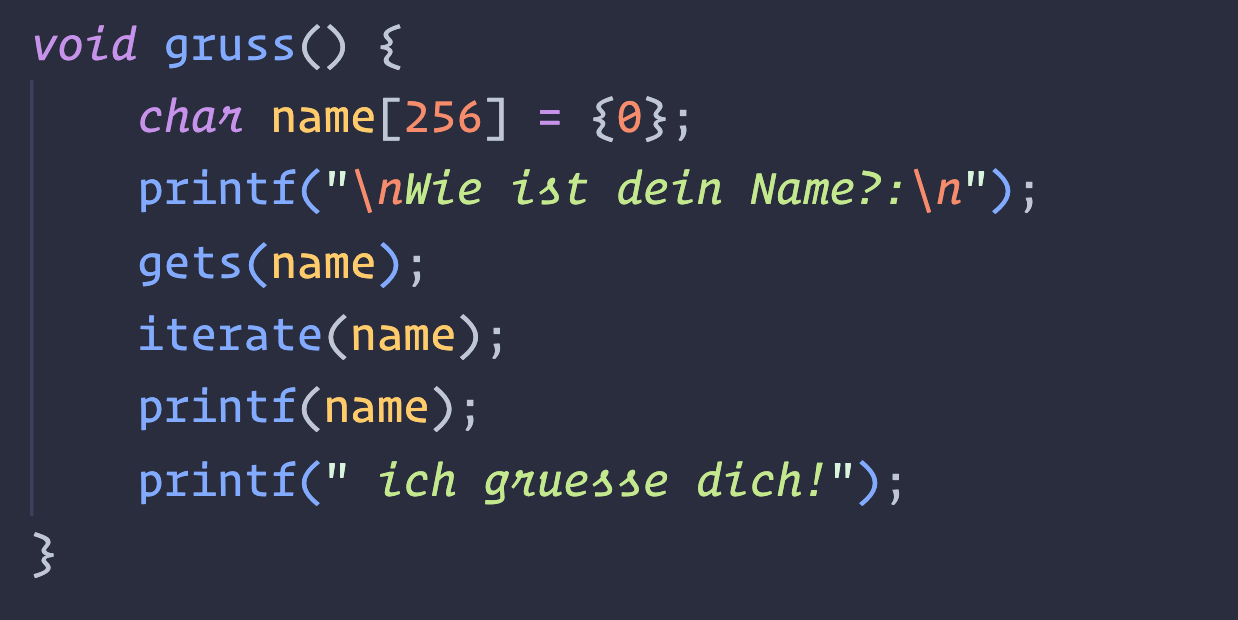
\includegraphics[width=0.7\textwidth,height=0.75\textheight,keepaspectratio]{images/gruss.png}
    \end{figure}
\end{frame}

\begin{frame}{Praktische Analyse}{Demonstration}
    \indent\hspace{5.5em}\large{Segmentierungsfehler}
    \begin{figure}[h]
        \centering
        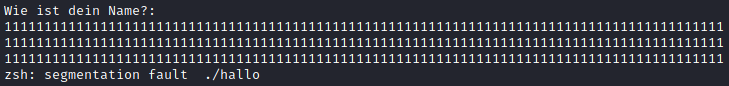
\includegraphics[width=0.7\textwidth,height=0.75\textheight,keepaspectratio]{images/segfault.png}
    \end{figure}
    \indent\hspace{5.1em}\large{Ausgegebene Speicheradressen}
    \begin{figure}[h]
        \centering
        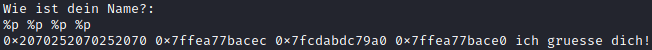
\includegraphics[width=0.7\textwidth,height=0.75\textheight,keepaspectratio]{images/adressen.png}
    \end{figure}
\end{frame}

\begin{frame}{Praktische Analyse}{Demonstration}
    \indent\hspace{5.4em}\large{Memory Map}
    \begin{figure}[h]
        \centering
        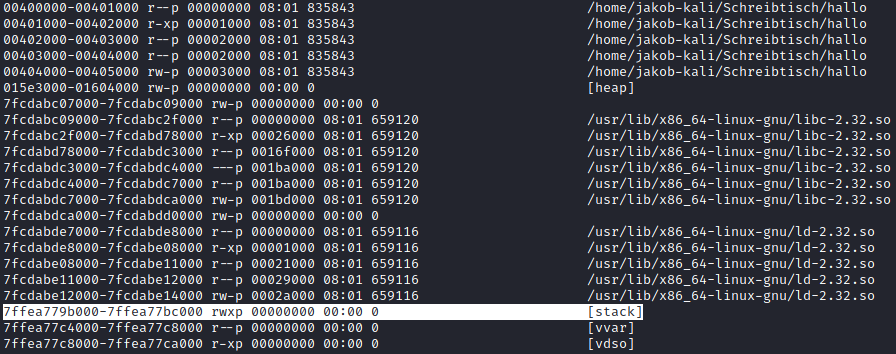
\includegraphics[width=0.7\textwidth,height=0.75\textheight,keepaspectratio]{images/map.png}
    \end{figure}
\end{frame}

    \begin{frame}{Praktische Analyse}{Demonstration}
    \indent\hspace{7.1em}\large{Speicherinhalt}
    \begin{figure}[h]
        \centering
        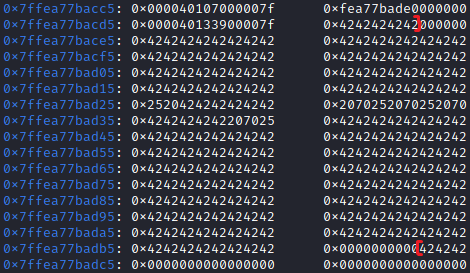
\includegraphics[width=0.6\textwidth,height=0.75\textheight,keepaspectratio]{images/buffer.png}
    \end{figure}
\end{frame}

\begin{frame}{Praktische Analyse}{Demonstration - Position des RIP}
    \begin{figure}[h]
        \centering
        
\includegraphics[width=0.8\textwidth,height=0.75\textheight,keepaspectratio]{images/characters.png}
    \end{figure}
\end{frame}

\begin{frame}{Praktische Analyse}{Demonstration - Payloads}
    \begin{figure}[h]
        \centering
        
\includegraphics[width=0.7\textwidth,height=0.75\textheight,keepaspectratio]{images/payload1.png}
    \end{figure}
    \begin{figure}[h]
        \centering
        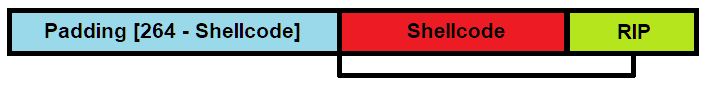
\includegraphics[width=0.7\textwidth,height=0.75\textheight,keepaspectratio]{images/payload2.png}
    \end{figure}
    \begin{figure}[h]
        \centering
        
\includegraphics[width=0.5\textwidth,height=0.75\textheight,keepaspectratio]{images/nop.png}
    \end{figure}
\end{frame}

\begin{frame}{Praktische Analyse}{Demonstration - Exploit}
    \begin{figure}[h]
        \centering
        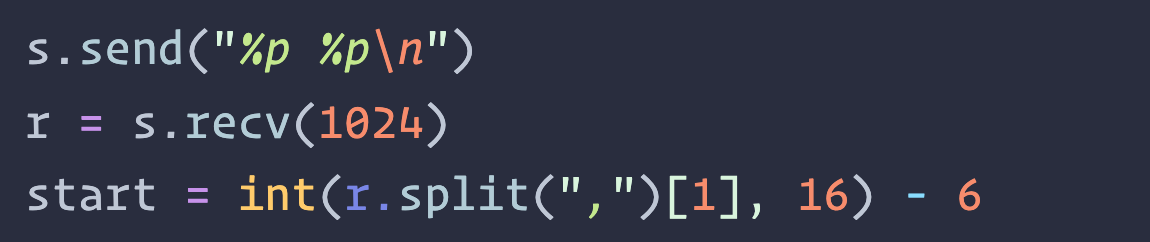
\includegraphics[width=0.5\textwidth,height=0.75\textheight,keepaspectratio]{images/format.png}
    \end{figure}
    \begin{figure}[h]
        \centering
        
\includegraphics[width=0.5\textwidth,height=0.75\textheight,keepaspectratio]{images/rip.png}
    \end{figure}
    \begin{figure}[h]
        \centering
        
\includegraphics[width=0.5\textwidth,height=0.75\textheight,keepaspectratio]{images/payload.png}
    \end{figure}
\end{frame}

\begin{frame}{Praktische Analyse}{Demonstration - Root Shell}
    \begin{figure}[h]
        \centering
        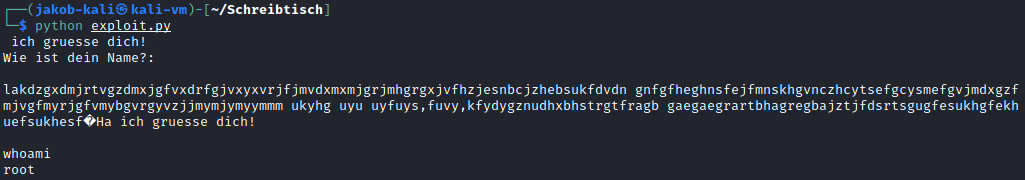
\includegraphics[width=1\textwidth,height=0.75\textheight,keepaspectratio]{images/root.png}
    \end{figure}
\end{frame}

